\section{Jet flavour tagging}
\label{sec:ch6_btag}

\subsection{Reconstruction inputs}

Jets containing $b$-hadrons are identified using the displacement of their decay products from the primary vertex.
With a typical proper lifetime of about $1.5$~ps, a boosted $b$-hadron can travel several millimetres before decaying~\cite{ATLAS2026GN2}.
Its charged decay products can therefore have significant impact parameters and a common secondary vertex.
The subsequent decay of a charm hadron can produce an additional displaced vertex.
The track momenta, impact parameters, detector hit information and correlations between tracks are used as flavour-tagging inputs.

\subsection{Identification}

The GN2v01 algorithm is used for $b$-tagging in this analysis.
Jet and track information is processed with a transformer neural network, in which the representation of each track is updated using information from other tracks in the jet~\cite{ATLAS2026GN2}.
Tracks with a common displaced origin can thereby be recognised together.
During training, auxiliary tasks are used to identify track origins and to group tracks from the same vertex, as illustrated in Figure~\ref{fig:ch6_gn2}.
Explicitly reconstructed secondary vertices are not required as separate input objects.

\begin{figure}[htbp]
    \centering
    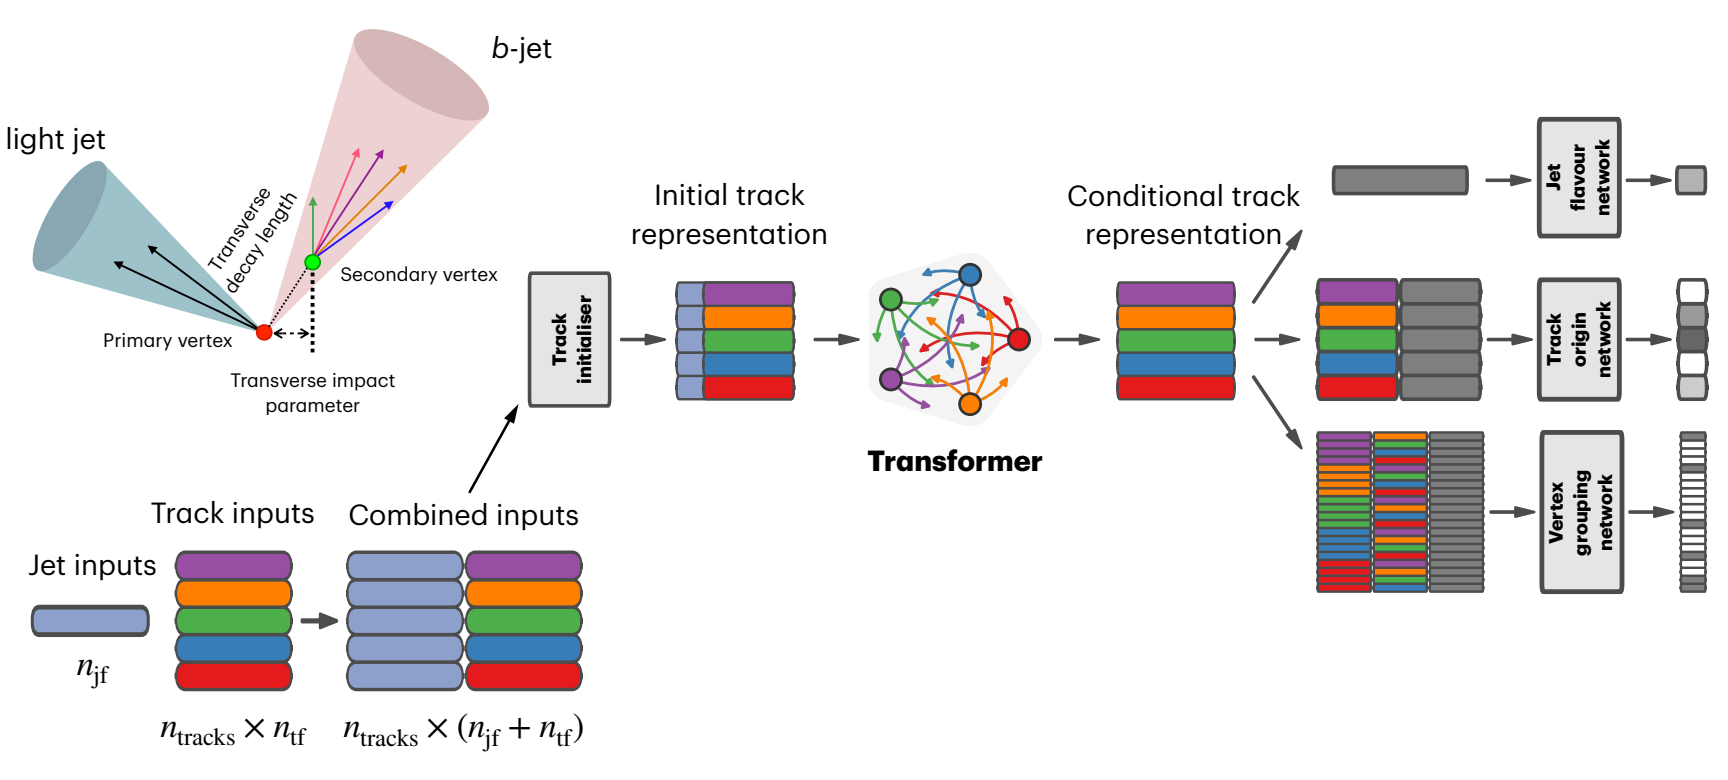
\includegraphics[width=\textwidth]{output/ch6/figures/gn2_architecture.png}
    \caption[GN2 flavour-tagging architecture]{GN2 flavour-tagging architecture. Jet and track measurements are combined, processed by the transformer, and used for jet-flavour prediction and the auxiliary track-origin and vertex-grouping tasks. The symbols $n_{\mathrm{jf}}$, $n_{\mathrm{tf}}$ and $n_{\mathrm{tracks}}$ denote the numbers of jet features, track features and tracks~\cite{ATLAS2026GN2}.}
    \label{fig:ch6_gn2}
\end{figure}

The outputs for the $b$-, $c$-, hadronic-tau and light-jet hypotheses are combined into the discriminant
\begin{align}
    D_b=\ln\!\left[
    \frac{p_b}{f_c p_c+f_\tau p_\tau+(1-f_c-f_\tau)p_u}
    \right],
    \label{eq:ch6_gn2_discriminant}
\end{align}
where $p_b$, $p_c$, $p_\tau$ and $p_u$ are the classifier outputs~\cite{ATLAS2026GN2}.
The fixed coefficients $f_c$ and $f_\tau$ set the balance between the background flavours in the discriminant.
A jet is tagged when $D_b$ exceeds the working-point threshold.
The nominal working point corresponds to an inclusive $b$-jet efficiency of 85\% in simulated $\ttbar$ events.
The efficiency for signal $b$-jets can differ because of their different kinematic distributions.
For a background flavour $f$, the rejection is defined as $1/\epsilon_f$, where $\epsilon_f$ is its probability of passing the tagging requirement.

\subsection{Calibration}

Tagging and mistagging efficiencies are measured in flavour-enriched data samples and compared with simulation~\cite{ATLAS2026GN2}.
Flavour- and kinematics-dependent scale factors are applied to simulated event weights.
Both tagged and untagged outcomes must be corrected.
For a single jet with tagging efficiency $\epsilon_f$, the correction for an untagged outcome is
\begin{align}
    w_f^{\mathrm{untagged}}
    =\frac{1-\epsilon_f^{\mathrm{data}}}{1-\epsilon_f^{\mathrm{MC}}}
    =\frac{1-\mathrm{SF}_f\epsilon_f^{\mathrm{MC}}}{1-\epsilon_f^{\mathrm{MC}}}.
    \label{eq:ch6_btag_untagged}
\end{align}
This complementary-probability relation explains why flavour-tagging corrections affect both the zero-tag and tagged event categories.
In this search, the zero-tag category also receives a direct contribution from $U_1\rightarrow s\tau$ when $\beta_L^{23}$ is sizeable, as discussed in Chapter~\ref{chapter:event_selection}.
